\documentclass[a4paper,10pt]{article}

%% Paquetes Adicionales %%

\usepackage[spanish]{babel}
\selectlanguage{spanish}
\spanishdecimal{.}
\addto\captionsspanish{\def\tablename{Cuadro}}
\usepackage{fancyhdr}
\usepackage{graphics}
\usepackage[dvips]{graphicx}
\usepackage[normal]{caption2}
\usepackage{amsfonts,amssymb,amsmath,amsthm}
\usepackage[T1]{fontenc}
\usepackage{moreverb}

%% Declaracion de comandos %%

\newtheorem{lema}{Lema}
\newtheorem{teor}{Teorema}
\newtheorem{propos}{Proposici\'on}
\newtheorem{corol}{Corolario}

\newcommand{\mivec}[1]{\mathbf{#1}}
\newcommand{\vers}[1]{\mivec{\check{#1}}}
\newcommand{\deriv}[2]{\frac{\mathrm{d}#1}{\mathrm{d}#2}}
\newcommand{\expo}[1]{~10^{#1}}
\newcommand{\uni}[1]{\mathrm{#1}} 

\newcommand{\prop}[1]{\begin{propos} #1 \end{propos}}
\newcommand{\teo}[1]{\begin{teor} #1 \end{teor}}
\newcommand{\cor}[1]{\begin{corol} #1 \end{corol}}
\newcommand{\lem}[1]{\begin{lema} #1 \end{lema}}

%% Encabezado y Pie de Pagina %%

\pagestyle{plain}
\lhead{}
\chead{}
\rhead{}
\cfoot{\thepage}
\renewcommand{\footrulewidth}{0.4pt}

%%\author{Juan Ignacio Go\~ni}

\makeindex

%% Titulo %%
\begin{document}
\title{{\ Taller de proyecto final \\ Robot recolector de residuos \\ Placa m\'odulo gen\'erico}}

%\date{}

%% Comienzo del documento %%

\maketitle

\begin{abstract}
En el presente se establecen las especificaciones para la placa del m\'odulo gen\'erico.
Se expone el circuito de la placa, explica funcionamiento y se muestran posibles usos.

\textbf{Palabras Clave: }\emph{Robot, residuos, protocolo, serial, rs-232, daisy chain}.
\end{abstract}

%\thispagestyle{fancy}

%% COMIENZO DEL TEXTO %%

\section{Introducci\'on}
\label{introduccion}

Durante el dise\~no de las placas controladoras surgi\'o la necesidad de establecer un m\'odulo com\'un de comunicaci\'on y una base de prueba
para los testeos con los distintos sensores y perif\'ericos que se utilizar\'ian en el robot.
Crear una placa que resuelva dichas cuestiones fue de gran ayuda y aceler\'o en gran medida las pruebas y dise\~no de las placas que le sucedieron.

En las siguientes secciones se detalla cada uno de los aspectos tenidos en cuenta para crear una placa gen\'erica para el desarrollo del robot.

\section{Microcontrolador}
\label{microcontrolado}

El microcontrolador elegido para la placa es el 16F88 de Microchip.
Cuenta con una memoria \emph{FLASH} para 4096 instrucciones de programa, una memoria \emph{RAM} de 368 bytes y una memoria \emph{EEPROM} de 256 bytes.
Cuenta con un reducido set de instrucciones b\'asicas todas con el mismo tiempo de ejecuci\'on.
En la subsecci\'on \ref{perifericos} se listan algunos de los principales perif\'ericos incluidos en el microcontrolador.
Se utiliza con un cristal externo de 20MHz como clock.

Para la carga y debug del firmware espec\'ifico para cada placa se utiliza el programador \emph{ICD2}, como se explica en la secci\'on \ref{programador}.

\subsection{Perif\'ericos}
\label{perifericos}

El microcontrolador 16F88 cuenta con 2 puertos de 8 entradas y salidas cada uno de tipo TTL y CMOS.
Cada pin se encuentra multiplexado con uno o m\'as perif\'ericos internos.

\subsubsection{Timers}
\label{timers}

Cuenta con 3 timers o contadores.

El \emph{TMR0} es de 8 bits y contiene un \emph{preescaler} de 8bits, es usado como WDT.
Tambi\'en puede ser utilizado como contador externo por el pin \emph{RA4}.

El \emph{TMR1} es de 16 bits y contiene un \emph{preescaler} de 2bits.
Puede ser utilizado como contador externo por el pin \emph{RB6} o con un cristal externo conectado a los pines \emph{RB6} y \emph{RB7}.

El \emph{TMR2} es de 8 bits, contiene un \emph{preescaler} de 2 bits y contiene un \emph{postscaler} de 4 bits.
Es de vital importancia para el m\'odulo de PWM por hardware.

\subsubsection{ADC}
\label{adc}

Cuenta con un conversor anal\'ogico digital de 8 o 10 bits multiplexado en 7 canales, 5 canales en el puerto A y 2 en el puerto B.
Es posible definir voltajes de referencia mediante ciertos pines o usar valores internos de referencia como \emph{Vcc} y \emph{GND}.

\subsubsection{PWM}
\label{pwm}

Cuenta con un m\'odulo de generaci\'on de un PWM por hardware de 10 bits de resoluci\'on con el ciclo y per\'iodo configurable mediante el \emph{TMR2}

\subsubsection{AUSART}
\label{ausart}

Cuenta con un m\'odulo de UART para comunicaci\'ion sincr\'onica o asincr\'onica utilizado para la implementaci\'on del daisy chain por RS-232.

\subsubsection{Otros}
\label{otros}

Para mayor informaci\'on respecto a los perif\'ericos o configuraci\'on del microcontrolador, se recomienda revisar las hojas de datos directo del fabricante.

\section{Comunicaci\'on}
\label{comunicacion}

El protocolo de comuncaci\'on est\'a formado por paquetes que representan un pedido de informaci\'on o comando que debe ser ejecutado en el destino.
Ver documentaci\'on del protocolo para mayor informaci\'on.

La comunicaci\'on est\'a basada en el m\'etodo \emph{Daisy chain} (patente US20090316836A1).
La cadena est\'a formada por las placas controladoras, las cuales se comunican entre ellas retransmitiendo cada paquete hacia adenlante.

\begin{figure}
\centering
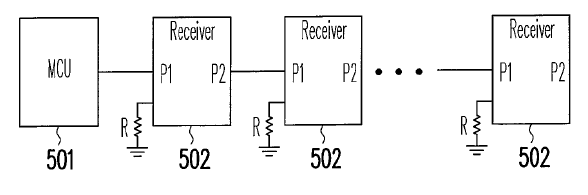
\includegraphics[scale=.5]{daisychain_diagram.png}
\caption{Diagrama general del m\'etodo daisy chain}
\label{daisychain_diagram}
\end{figure}

Como parte de la configuraci\'on de la placa, existe un switch que determina el tipo de eslab\'on de la placa (modo \emph{LINK}), si es un nodo intermedio
o la punta de la cadena (modo \emph{LAST}).

En la figura \ref{rj11db9} se muestran los conectores utilizados. En los cuadros \ref{conexionLink} y \ref{conexionRS232} se especifica el conexionado entre placas y contra el controlador principal.

\begin{figure}
\centering
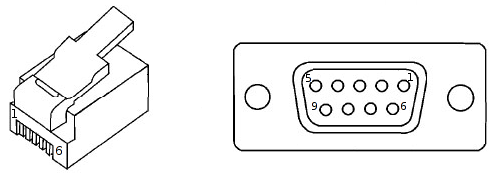
\includegraphics[scale=.5]{rj11_db9.png}
\caption{Conectores RJ11 y DB9 utilizados para la comuncaci\'ion}
\label{rj11db9}
\end{figure}

\begin{table}
\begin{center}
\begin{tabular}{|c|c|c|c|}
\hline
Funci\'on & Conector RJ11 & Conector RJ11 & Funci\'on\\
\hline
Serial RX & 2 & 2 & Serial TX \\
\hline
Serial TX & 3 & 3 & Serial RX \\
\hline
No conectado & 4 & 4 & No conectado \\
\hline
GND & 5 & 5 &  GND\\
\hline
\end{tabular}
\caption{Conexionado entre placas en modo Link}
\label{conexionLink}
\end{center}
\end{table}

\begin{table}
\begin{center}
\begin{tabular}{|c|c|c|c|}
\hline
Funci\'on & Conector RJ11 & Conector DB9 & Funci\'on\\
\hline
Serial RX & 2 & 3 & Serial TX \\
\hline
Serial TX & 3 & 2 & Serial RX \\
\hline
No conectado & 4 & 4 & Shield \\
\hline
GND & 5 & 5 &  GND\\
\hline
\end{tabular}
\caption{Conexionado entre placa y la PC}
\label{conexionRS232}
\end{center}
\end{table}

Se recomienda el uso de cable de par trenzado o mallado para disminuir la interferencia.

\section{Alimentaci\'on}
\label{alimentacion}

La alimentaci\'on principal de la placa es 7 a 20 voltios, con la posibilidad de alimentarla directamente 
con 5 voltios por uno de los pines del conector. 
En la figura \ref{borneras} se muestra la bornera y en el cuadro \ref{alimentacionLogica} el pinout de la misma.

\begin{figure}
\centering
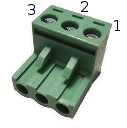
\includegraphics[scale=.5]{bornera3.png}
\caption{Bornera de 3 pines para la alimentaci\'on de la placa}
\label{borneras}
\end{figure}

\begin{table}
\begin{center}
\begin{tabular}{|c|c|}
\hline
Pin & Voltaje \\
\hline
1 & GND \\
\hline
2 & 5v \\
\hline
3 & 7v a 12v \\
\hline
\end{tabular}
\caption{Alimentaci\'on de la l\'ogica}
\label{alimentacionLogica}
\end{center}
\end{table}

La regulaci\'on interna de voltaje realiza por medio de un regulador 7805 corriente m\'axima de 1A.

\section{Configuraci\'on}
\label{configuracion}

El header de programaci\'on \emph{P1} se utiliza para conectar la placa con el programador y debuguer de c\'odigo \emph{ICD2} como se explica en la secci\'on \ref{programador}.

La fila de pines \emph{P2} exporta todos los pines con funciones dentro del microcontrolador, para realizar conexiones con perif\'ericos de prueba.
Los headers \emph{P3} y \emph{P4} son jumpers que vinculan los pines \emph{RA1} y \emph{RA4} del microcontrolador los leds 1 y 2 respectivamente.

El switch \emph{S3} como se explica en la secci\'on \ref{comunicacion}, se utiliza para determinar el papel de la placa dentro de la cadena (modo \emph{LINK} o modo \emph{LAST}).
El switch \emph{S2} se utiliza para asociar los pines del microcontrolador con los canales de clock y data del header de programaci\'on (modo \emph{ICD2}) o con los pines del header \emph{P2}.


\section{Posibles usos}
\label{usos}

Desde el principio, la placa fue pensada como una placa es el testeo de la comunicaci\'on y conexionado de nuevos perif\'ericos y sensores.
Aunque tambi\'en puede ser usada como placa entrenadora para proveer un punto de entrada a nuevos integrantes del proyecto en la programaci\'on de placas y nuevos sensores.

Ultilizada mayormente en la etapa de dise\~no, disminuye los errores y posibilita el concentrarse en las partes nuevas con las que se est\'a trabajando.

\section{Esquem\'atico}
\label{esquematico}

En la figura \ref{schema1} se detalla el esquem\'atico del microcontrolador y el conexionado con los headers.

En la figura \ref{schema2} se muestra el m\'odulo de comunicaci\'on y el conexionado con los conectores para conformar la cadena \emph{Daisy chain}.

En la figura \ref{schema3} se muestra la fuente de alimentaci\'on y bornera.

\begin{figure}
\centering
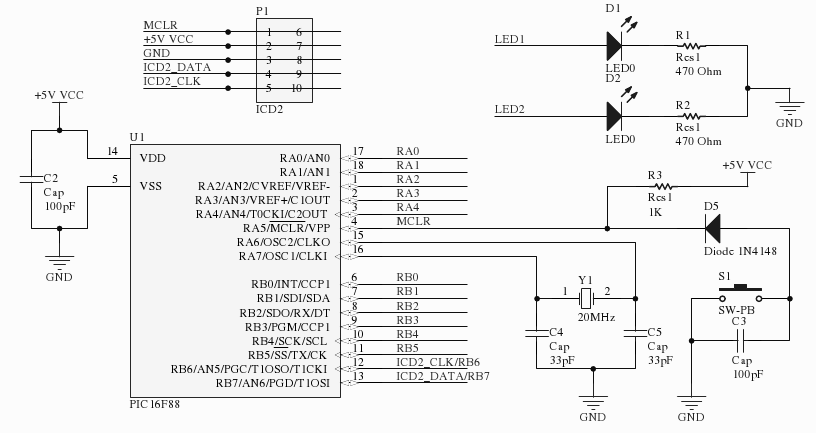
\includegraphics[scale=.3]{schemaMicro.png}
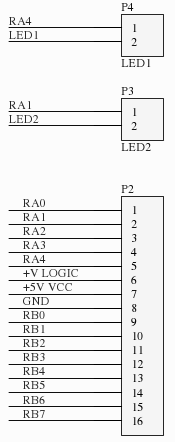
\includegraphics[scale=.3]{schemaHeaders.png}
\caption{Microcontrolador y headers}
\label{schema1}
\end{figure}

\begin{figure}
\centering
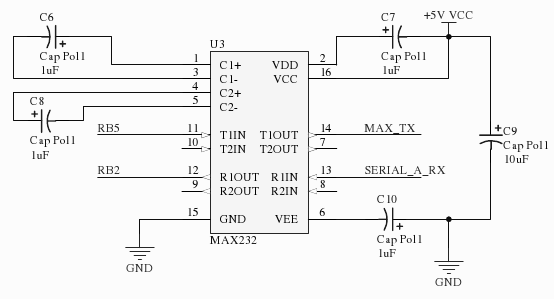
\includegraphics[scale=.3]{schemaComm1.png}
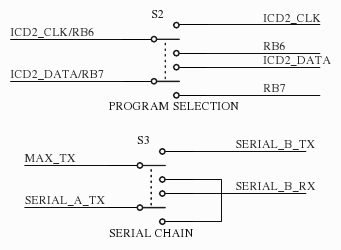
\includegraphics[scale=.3]{schemaComm2.png}
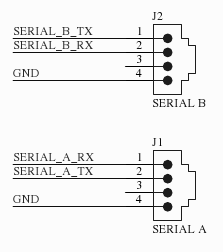
\includegraphics[scale=.3]{schemaComm3.png}
\caption{Comunicaci\'on, switch de modo y conectores de entrada y salida}
\label{schema2}
\end{figure}

\begin{figure}
\centering
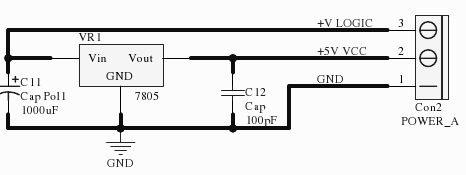
\includegraphics[scale=.3]{schemaFuente.png}
\caption{Fuente de alimentaci\'on}
\label{schema3}
\end{figure}

\section{Circuito}
\label{circuito}

En la figura \ref{componentes} se muestra la m\'ascara de componentes de la placa.
En la figura \ref{capas} se muestran ambas capas de la placa.

\begin{figure}
\centering
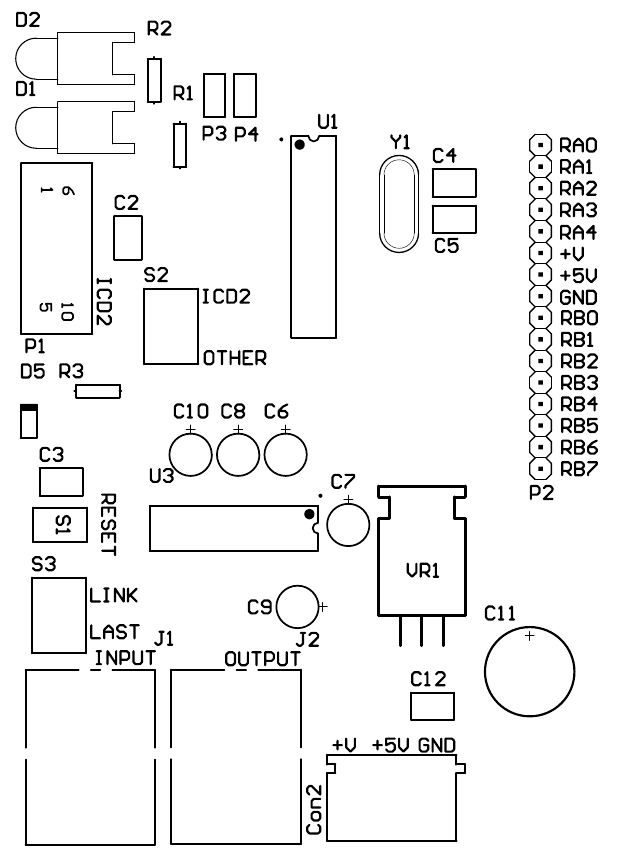
\includegraphics[scale=.2]{componentes.png}
\caption{M\'ascara de componentes}
\label{componentes}
\end{figure}

\begin{figure}
\centering
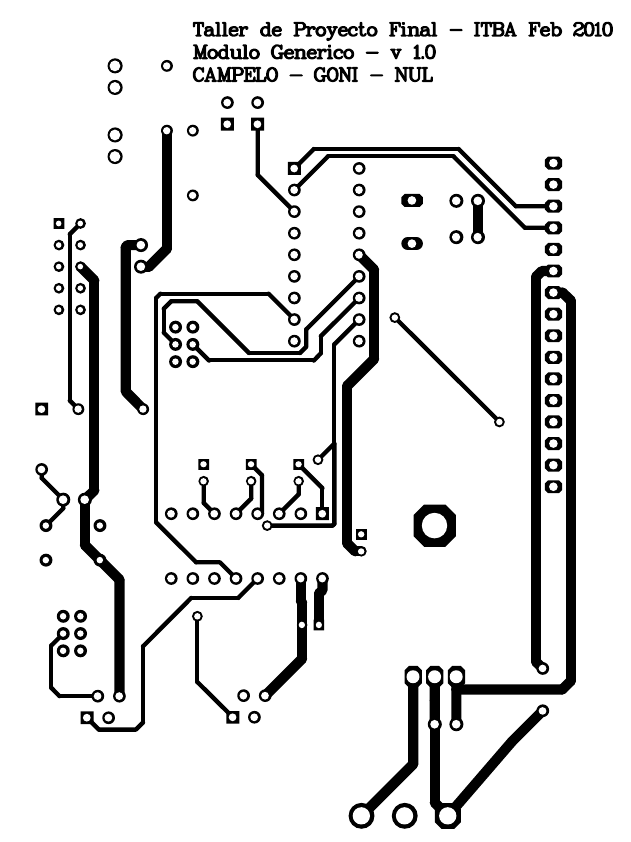
\includegraphics[scale=.2]{top.png}
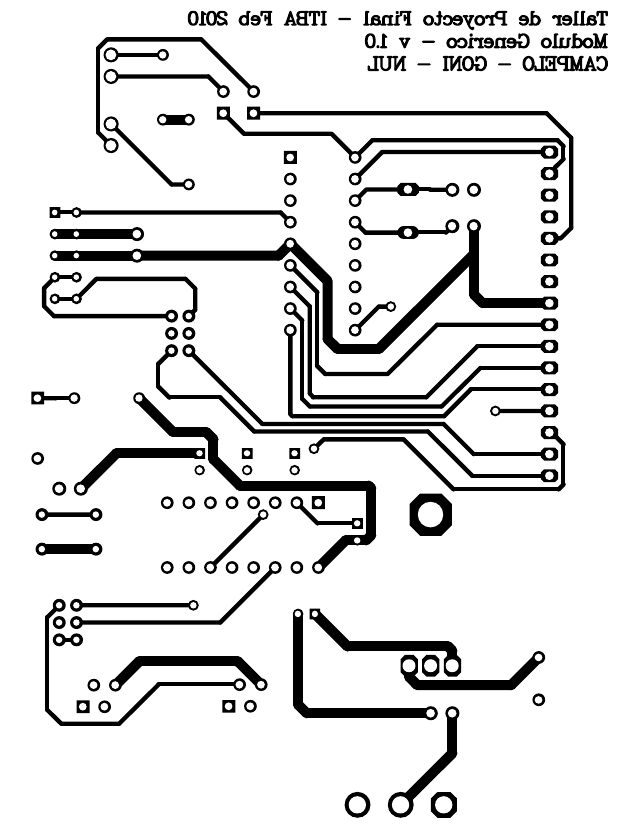
\includegraphics[scale=.2]{bottom.png}
\caption{Capas superior e inferior de la placa}
\label{capas}
\end{figure}


\section{El programador}
\label{programador}

El programador utilizado es el modelo \emph{ICD2} de la empresa \emph{Microchip}.
Provee una interfaz tanto para la carga y descarga de firmware al microcontrolador, sino que tambi\'en permite debuguear dicho c\'odigo.

La IDE de programaci\'on utilizada es \emph{Microchip MPLAB} debido a su completa integraci\'on con el producto.

El lenguaje de programaci\'on utilizado es \emph{C} y el compilador elegido es \emph{CCS PCM V4.023}.

\section{C\'odigo b\'asico}
\label{codigo}

Debido a que la placa fue pensada como punto de partida, se provee del c\'odigo utilizado como base para la programaci\'on de las otras placas controladoras.

{\scriptsize
\begin{verbatimtab}
#define CARD_GROUP	MOTOR_DC	// Ver protocol.h
#define CARD_ID		0		// Valor entre 0 y E

// Descripcion de la placa
#define DESC		"PLACA GENERICA - 1.0" // Maximo DATA_SIZE bytes

/* Modulo Generico - main.c
 * PIC16F88 - MAX232 - GENERICO
 *
 *                               PIC16F88
 *                .------------------------------------.
 *               -|RA2/AN2/CVREF/VREF           RA1/AN1|- LED
 *               -|RA3/AN3/VREF+/C1OUT          RA0/AN0|- 
 *           LED -|RA4/AN4/T0CKI/C2OUT    RA7/OSC1/CLKI|- XT CLOCK pin1, 27pF to GND
 * RST/ICD2:MCLR -|RA5/MCLR/VPP           RA6/OSC2/CLKO|- XT CLOCK pin2, 27pF to GND
 *           GND -|VSS                              VDD|- +5v
 *               -|RB0/INT/CCP1       RB7/AN6/PGD/T1OSI|- ICD2:PGD/
 *               -|RB1/SDI/SDA  RB6/AN5/PGC/T1OSO/T1CKI|- ICD2:PGC/
 *  MAX232:R1OUT -|RB2/SDO/RX/DT           RB5/SS/TX/CK|- MAX232:T1IN
 *               -|RB3/PGM/CCP1             RB4/SCK/SCL|- 
 *                '------------------------------------'
 *    
 */

#include <16F88.h>
#DEVICE ADC = 10
#include <stdio.h>
#include <string.h>
#include <stdlib.h>

#fuses HS,NOWDT,NOPROTECT,NOLVP
#use delay (clock=20000000)

#use rs232(BAUD=115200,PARITY=N,XMIT=PIN_B5,RCV=PIN_B2,BITS=8,ERRORS,TIMEOUT=1,STOP=1,UART1)
#use fast_io(A)
#use fast_io(B)

#byte porta=0x05
#byte portb=0x06

// Led
#bit led1=porta.1
#bit led2=porta.4

// MAX232
#bit tx=portb.5
#bit rx=portb.2

#include <../../protocolo/src/protocol.c>
/*
** Variables definidas en protocol.c

short reset; // Variable para hacer el reset
short crcOK; // Informa si el CRC del paquete parseado fue correcto
short sendResponse; // Informa que no debe mandarse la respuesta automatica

char buffer[MAX_BUFFER_SIZE];	// Buffer de recepcion de comandos
int buffer_write;		// Indice de escritura
int buffer_read;		// Indice de lectura
int data_length;		// Largo de los datos en el buffer

struct command_t command; 	// Comando parseado
struct command_t response; 	// Respuesta

** Implementar las siguientes funciones (usadas por el protocolo)

void init(); // Inicializa puertos y variables
void doCommand(struct command_t * cmd); // Examina y ejecula el comando

***/

void init()
{
	// Inicializa puertos
	set_tris_a(0b11100101);
	set_tris_b(0b11100110);

	// Variable para hacer el reset
	reset = false;

	return;	
}	

void main()
{
	// Placa Generica - Implementacion del protocolo
	init();

	// Init del protocol
	initProtocol();

	// FOREVER
	while(true)
	{
		// Hace sus funciones...

		// Protocolo
		runProtocol(&command);
	}

	return;
}

/* Verifica que el comando sea valido y lo ejecuta */
void doCommand(struct command_t * cmd)
{
	int crc, i, len;
		
	// Calculo del CRC
	crc = generate_8bit_crc((char *)cmd, cmd->len, CRC_PATTERN);
	
	// CRC ok?
	if (cmd->crc != crc)
	{		
		// Creo respuesta de error
		response.len = MIN_LENGTH + cmd->len + 2 + 1;
		response.to = cmd->from;
		response.from = THIS_CARD;
		response.cmd = COMMON_ERROR;
		response.data[0] = 0x00;
		// Agrego el paquete que contiene el error de CRC
		response.data[1] = cmd->len;
		response.data[2] = cmd->to;
		response.data[3] = cmd->from;
		response.data[4] = cmd->cmd;
		// Campo data
		len = cmd->len - MIN_LENGTH;
		for (i = 0; i < len; i++)
			response.data[5 + i] = (cmd->data)[i];
		// CRC erroneo
		response.data[5 + len] = cmd->crc;
		// CRC esperado
		response.data[5 + len + 1] = crc;
		// CRC de la respuesta
		response.crc = generate_8bit_crc((char *)(&response), response.len, CRC_PATTERN);
	
		crcOK = false;
		return;
	}

	crcOK = true;
	
	// Minimo todos setean esto
	response.len = MIN_LENGTH;
	response.to = cmd->from & 0x77;
	response.from = THIS_CARD;
	response.cmd = cmd->cmd | 0x80;

	switch (cmd->cmd)
	{
		// Comandos comunes
		case COMMON_INIT: 
			init();
			// Enviar la descripcion de la placa en texto plano
			strcpy(response.data, DESC);
			response.len += strlen(response.data);
		break;
		case COMMON_RESET: 
			// Enviar la descripcion de la placa en texto plano
			strcpy(response.data, DESC);
			response.len += strlen(response.data);
			// Reset!
			reset = true;
		break;
		case COMMON_PING: 
			// No hace falta hacer mas nada
		break;
 		case COMMON_ERROR:
			// Por ahora se ignora el comando
		break;
		
		/* Comandos especificos */

 		case 0x40:
			/* 
			:DATO:
			-
			:RESP:
			-
			*/
		break;

		default:
			response.len++;
			response.cmd = COMMON_ERROR;
			response.data[0] = 0x01; // Comando desconocido
		break;
	}	

	// CRC de la respuesta
	response.crc = generate_8bit_crc((char *)(&response), response.len, CRC_PATTERN);

	return;
}
\end{verbatimtab}
}

El c\'odigo incluye al archivo \emph{protocolo.c} que se muestra a continuaci\'on.

{\scriptsize
\begin{verbatimtab}
#include <../../protocolo/src/protocol.h>

short reset;
short crcOK;
short sendResponse;

char buffer[MAX_BUFFER_SIZE];
int buffer_write;
int buffer_read;
int data_length;

// Comando parseado
struct command_t command;
// Respuesta
struct command_t response;

// Interrupcion del RS232
#INT_RDA
void RS232()
{
	disable_interrupts(INT_RDA);
	// Un nuevo dato...
	buffer[buffer_write++] = getc();
	data_length++;
	if (buffer_write == MAX_BUFFER_SIZE)
		buffer_write -= MAX_BUFFER_SIZE;
	enable_interrupts(INT_RDA);
	return;
}

/* Envia los datos por el pto serial */
void initProtocol()
{
	// Variables de comunicacion
	buffer_write = 0;
	buffer_read = 0;
	data_length = 0;
	crcOK = false;
	
	// Interrupcion Rcv
	enable_interrupts(INT_RDA);

	// Habilito las interrupciones
	enable_interrupts(GLOBAL);
}

/* Envia los datos por el pto serial */
void send(struct command_t * cmd)
{
	int i, len;
	
	len = cmd->len - 4;
	putc(cmd->len);
	putc(cmd->to);
	putc(cmd->from);
	putc(cmd->cmd);
	
	for (i = 0; i < len; i++)
	{
		putc((cmd->data)[i]);
	}
	
	// Enviar el CRC
	putc(cmd->crc);
	
	return;	
}	

void runProtocol(struct command_t * cmd)
{
	// Analiza el buffer
	if (buffer[buffer_read] < data_length)
	{
		data_length -= buffer[buffer_read] + 1;
	
		cmd->len = buffer[buffer_read++];
	
		if (buffer_read == MAX_BUFFER_SIZE)
			buffer_read = 0;
	
		cmd->to = buffer[buffer_read++];
	
		if (buffer_read == MAX_BUFFER_SIZE)
			buffer_read = 0;
	
		cmd->from = buffer[buffer_read++];
	
		if (buffer_read == MAX_BUFFER_SIZE)
			buffer_read = 0;
	
		cmd->cmd = buffer[buffer_read++];
	
		if (buffer_read == MAX_BUFFER_SIZE)
			buffer_read = 0;
	
		// Obtiene el campo DATA
		if ((buffer_read + cmd->len - MIN_LENGTH) > MAX_BUFFER_SIZE)
		{
			// DATA esta partido en el buffer ciclico
			memcpy(cmd->data, buffer + buffer_read, MAX_BUFFER_SIZE - buffer_read);
			memcpy(cmd->data + MAX_BUFFER_SIZE - buffer_read, buffer, 
				cmd->len - MIN_LENGTH - MAX_BUFFER_SIZE + buffer_read);
		} else {
			// DATA esta continuo
			memcpy(cmd->data, buffer + buffer_read, cmd->len - MIN_LENGTH);
		}
	
		buffer_read += cmd->len - MIN_LENGTH;
		if (buffer_read >= MAX_BUFFER_SIZE)
			buffer_read -= MAX_BUFFER_SIZE;
	
		cmd->crc = buffer[buffer_read++];
	
		if (buffer_read == MAX_BUFFER_SIZE)
			buffer_read = 0;

		sendResponse = true;

		// Soy el destinatario?
		if (cmd->to == THIS_CARD)
		{
			// Ejecuta el comando
			doCommand(cmd);
		} else // Es broadcast?
			if ((cmd->to & 0xF0) == 0xF0)
		{
			// Ejecuta el comando
			doCommand(cmd);

			if (crcOK == true)
			{
				// Envia la respuesta
				send(&response);
				// Envia nuevamente el comando recibido
				response = *cmd;
			}
		} else // Es broadcast para mi grupo? 
			if (((cmd->to & 0x0F) == 0x0F) &&
			 	((cmd->to & 0xF0) == THIS_GROUP))
		{
			// Ejecuta el comando
			doCommand(cmd);	
#ifdef RESEND_GROUP_BROADCAST
			if (crcOK == true)
			{
				// Envia la respuesta
				send(&response);
				// Envia nuevamente el comando recibido
				response = *cmd;
			}
#endif
		} else {
			response = *cmd;
		}
	
		// Envia la respuesta?
		if (sendResponse == true)
		{
			send(&response);
		}	

	}
	
	// Reset del micro
	if (reset == true)
	{
		reset_cpu();
	}	

}

int generate_8bit_crc(char* data, int length, int pattern)
{
	// TODO: reemplazar por el crc?
	
	int crc_byte, i;

	crc_byte = data[0];
			
	for (i = 1; i < length; i++)
		crc_byte ^= data[i];
	
	return crc_byte;
}
\end{verbatimtab}
}

\end{document}